\section{Alhazenov problem}

Spoznajmo zanimiv problem, ki izhaja že iz stare Grčije. Čez poglavje si bomo pogledali več njegovih različic in poskusili najti origami konstrukcijo njegove rešitve.

\subsubsection*{Starogrški izvor problema}

V osnovi gre za problem s področja optike, ki naj bi ga zastavil grški matematik Ptolemaj (prb.\ 85--170 po Kr.): \emph{Pri danem sferičnem zrcalu in viru svetlobnega žarka poišči točko na zrcalu, od katere se bo svetlobni žarek odbil v oko opazovalca} (slika~\ref{fig:ptolemaj}).

\begin{figure}[h]
    \centering
    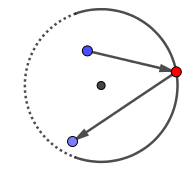
\includegraphics[width=0.25\textwidth]{images/alhazen/ptolemajev_problem.png}
    \caption[Ptolemajev problem]{Ptolemajev optični problem.}
    \label{fig:ptolemaj}
\end{figure}

Rešitev se da preformulirati v iskanje točke na krožnici, v kateri polmer krožnice razpolavlja kot, ki ga opravi svetlobni žarek. To velja zaradi \emph{odbojnega zakona}, vendar tega v takratni Grčiji še niso poznali. Pojdimo na začetek in opazujmo, kako se je oblika Ptolemajevega problema spreminjala skozi čas.

Grški matematik Heron iz Aleksandrije, med drugim znan po Heronovi formuli za izračun ploščine trikotnika z danimi dolžinami stranic, je okoli leta 100 po Kr.\ zastavil in rešil naslednje vprašanje, ki je različica Ptolemajevega problema: \emph{Na isti strani premice ležita točki $A$ in $B$. Poišči točko $C$ na premici, da bo pot od točke $A$ do $B$ preko točke $C$ najkrajša} (predpostavimo evklidsko metriko).

Sam točko $C$ konstruira zelo enostavno -- najprej točko $B$ zrcali čez premico v točko $B'$, nato pa s točko $C$ označi presečišče premice in daljice $AB'$ (slika~\ref{fig:heron}). Ker velja $|CB| = |CB'|$, je $|AC| + |CB| = |AC| + |CB'| = |AB'|$. Dolžina $|AB'|$ najkrajša možna razdalja med točkama $A$ in $B'$, zato je točka $C$ rešitev vprašanja.

\begin{figure}[h]
    \centering
    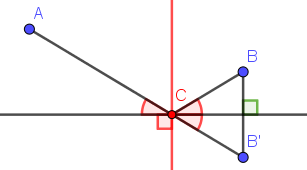
\includegraphics[width=0.4\textwidth]{images/alhazen/heron.png}
    \caption[Heronovo vprašanje]{Heronova konstrukcija najkrajše poti od točke $A$ do točke $B$.}
    \label{fig:heron}
\end{figure}

Zgornja konstrukcija pa je Heronu ponudila še nekaj -- opazil je, da pravokotnica na premico skozi točko $C$ namreč razpolavlja kot $\angle ACB$. Tako lahko njegovo vprašanje preoblikujemo v: \emph{Na isti strani premice ležita točki $A$ in $B$. Poišči točko $C$ na premici, ki razpolavlja kot $\angle ACB$.}

\opomba{Bralcu je za vajo prepuščen enostaven premislek, kako konstruirati točko $C$ z origamijem.}

\subsubsection*{Formulacija Alhazenovega problema}

S tem novim znanjem je Heron postavil temelje, na katerih je več stoletij kasneje matematik, astronom in fizik Ibn al-Haytham oz.\ po naše Alhazen (prb.\ 965--1040), ki je živel na območju današnjega Iraka, formuliral odbojni zakon, ki pravi, da sta vpadni in odbojni kot žarka svetlobe od površja enaka. Alhazen se je tudi prvi bolj poglobil v Ptolemajev problem in prišel do pomembnih ugotovitev, zato problem ponekod imenujejo tudi Ptolemaj-Alhazenov problem, bolj pa je znan pod imenom \emph{Alhazenov problem} ali \emph{biljardni problem}\footnote{Ime izhaja iz iskanja točke na robu biljardne mize, kamor želimo poslati biljardno kroglo, da se odbije v želeno smer. V našem primeru je biljardna miza okrogle oblike namesto pravokotne.}. 

Zopet formulirajmo problem. Namesto premice imamo torej krožnico $\mathcal{K}$ s središčem $O$. Naj točki $A$ in $B$ ležita znotraj krožnice (za točki zunaj krožnice k reševanju problema postopamo na analogen način, je pa Alhazen originalno resda predpostavil ta položaj). Iščemo točko $C$ na krožnici $\mathcal{K}$, da se bo svetlobni žarek iz točke $A$ v točki $C$ odbil v točko $B$. Na enak način kot Heron lahko premislimo, da mora polmer $OC$ razpolavljati kot $ACB$ (slika~\ref{fig:alhazen1}).

\begin{figure}[h]
    \centering
    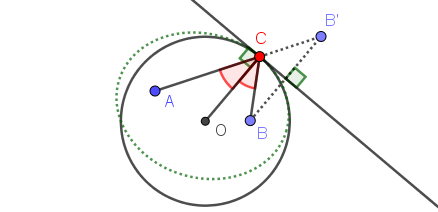
\includegraphics[width=0.6\textwidth]{images/alhazen/alhazen1.png}
    \caption[Alhazenov problem]{Ena od rešitev Alhazenovega problema v splošnem.}
    \label{fig:alhazen1}
\end{figure}

Za razliko od Heronove konstrukcije tu ne znamo konstruirati točke $B'$, saj je premica, čez katero bi morali zrcaliti točko $B$ (in tako s presečiščem daljice $AB'$ in premice dobiti točko $C$), ravno tangenta v točki $C$. Premice torej ne moremo dobiti brez točke $C$, točke $C$ pa ne moremo dobiti brez te premice. Tu se pokaže razsežnost problema in zazdeva se nam, da tudi origami konstrukcija tu ne bo enostavna.

Seveda so rešitve v nekaterih posebnih primerih enostavne -- če sta točki $A$ in $B$ enako oddaljeni od središča $O$, je točka $P$ presečišče simetrale daljice $AB$ oz. kota $\angle AOB$ s krožnico. V nadaljevanju bomo obravnavali le še en poseben primer, pri katerem obstaja zelo enostavna origami konstrukcija rešitve, sicer pa predpostavljamo splošno lego točk $A$ in $B$.

\opomba{Opazimo lahko tudi, da ima zaradi enakega vpadnega in odbojnega kota žarka v točka $C$ lastnost točke, ki leži na \emph{elipsi} z goriščema $A$ in $B$ (na sliki~\ref{fig:alhazen1} označena s prekinjeno črto). Tangenta na krožnico v točki $C$ je hkrati tudi tangenta na elipso v isti točki, torej lahko problem preoblikujemo v iskanje elipse z goriščema v $A$ in $B$, ki so tangentne na krožnico $\mathcal{K}$. Vendar ne poznamo enostavnega postopka, ki bi nam lahko poiskal enačbo te elipse, saj je ta odvisna od točke $C$, ta pa od tangente in obratno. Torej smo zopet na istem. Bralec, ki se želi poglobiti v reševanje Alhazenovega problema z elipsami, si lahko več o tem prebere v~\cite{masayo2019} in~\cite[str.\ 26--46]{gorjup2014}.}

Že tisoč let nazaj je Alhazen pokazal, da se da problem rešiti geometrijsko preko stožnic in da število rešitev variira od nič do največ štiri. Njegov dokaz je zelo obsežen in bil za marsikoga zelo zapleten in predolg~\cite{wilk2015}, zato je veliko matematikov za njim poskušalo poiskati enostavnejšo rešitev npr.\ preko kompleksnih števil in analitičnih metod v geometriji.

Leta 1672 je tako Huygens pokazal, da je Alhazenova rešitev ekvivalentna iskanju presečišča dane krožnice s hiperbolo (glej~\cite{nishimura2018}). Algebraično rešitev problema je l.\ 1965 našel Jack M.\ Elkin, ko je problem prevedel v reševanje enačbe četrte stopnje, ki jo lahko rešimo z računalnikom. Oboje si bomo pogledali v nadaljevanju. Alperin je v~\cite{alperin2002} izpostavil, da je potemtakem problem rešljiv z origamijem. Leta 1997 je Peter M.\ Neumann dokazal, da ne obstaja evklidska konstrukcija rešitve, kar sicer vemo že iz Elkinovega rezultata.

Problem se da posplošiti tudi na iskanje primerne točke odboja na zrcalu parabolične, eliptične in hiperbolične oblike, kar algebraično privede do reševanja enačbe največ osme stopnje~\cite{alhproblemwiki}. Skozi čas se je (vsaj za osnovni Alhazenov problem) razvilo še več različnih pristopov reševanja, vendar se bomo tu osredotočili na Huygensov nastavek, ki ga je japonski matematik Nishimura preko dualnih stožnic razširil na področje origamija.

\subsubsection*{Prevedba problema na reševanje kvartične enačbe}

Poglejmo, kako lahko Alhazenov problem prevedemo v reševanje enačbe četrte stopnje. Naslednji nastavek za izpeljavo enačbe je vzet iz~\cite[138--139]{geometricconstructions}. Brez škode za splošnost predpostavimo, da je krožnica $\mathcal{K}$ enotska, $O = (0,0), A = (0,a)$ in $B=(b,c)$ za take $0 \leq a, b, c \leq 1$, da te točke med sabo paroma ne sovpadajo (slika~\ref{fig:alhazen2}). Naj bo $C=(x,y)$ iskana točka na krožnici $\mathcal{K}$. Iz tega sledi pogoj
\begin{equation}
    \label{eq:pogoj_alh1}
    x^2 + y^2 = 1.
\end{equation}

\begin{figure}[h]
    \centering
    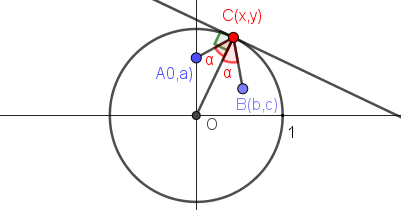
\includegraphics[width=0.6\textwidth]{images/alhazen/alhazen2.png}
    \caption[Alhazenov problem -- izpeljava]{Podlaga za izpeljavo kvartične enačbe za Alhazenov problem.}
    \label{fig:alhazen2}
\end{figure}

Naj bodo premice $AC$, $OC$ in $BC$ nosilke istoimenskih daljic in naj bo za vsako premico $i$ s $k_i$ označen njen koeficient. Dobimo
$$ k_{AC} = \frac{y-a}{x}, \; k_{OC} = \frac{y}{x} \; \text{ in } \; k_{BC} = \frac{y-c}{x-b}.$$
Označimo $\alpha = \angle ACO = \angle OCB$. Ker sta kota enaka, velja
\begin{align*}
    \tan \alpha &= tan \alpha, \\
    \frac{k_{AC} - k_{OC}}{1 + k_{AC} k_{OC}} &= \frac{k_{OC} - k_{BC}}{1 + k_{OC} k_{BC}}, \\
    \frac{\frac{y-a}{x} - \frac{y}{x}}{1 + \frac{y-a}{x} \cdot \frac{y}{x}} &= \frac{\frac{y}{x} - \frac{y-c}{x-b}}{1 + \frac{y}{x} \cdot \frac{y-c}{x-b}}.
\end{align*}
Slednjo enačbo poenostavimo in z upoštevanjem pogoja~\ref{eq:pogoj_alh1} dobimo
$$ y(b + 2acx) = ab + (a+c)x - 2abx^2.$$
Enačbo kvadriramo, spet upoštevamo pogoj~\ref{eq:pogoj_alh1} in dobimo enačbo četrte stopnje (\textcolor{red}{si poračunala, tudi z wolframom, je na enem listu}):
$$ 4a^2(b^2 + c^2)x^4 - 4a^2bx^3 + (a^2 - 4a^2b^2 + b^2 + c^2 - 4a^2c^2 + 2ac)x^2 + 2ab(a-c)x + b^2(a^2-1) = 0.$$

Enačbe četrte stopnje v teoriji znamo rešiti tako računsko kot z origamijem, vendar je to praktično precej zapleteno in delo raje prepustimo računalniku.

\subsubsection*{Origami konstrukcija rešitve za poseben primer}

Za poseben primer izbire točk $A$ in $B$ pri dani krožnici na naše veselje vendarle obstaja zelo enostavna konstrukcija točke $C$. Scimemi v~\cite[str.\ 116-117]{scimemi2002} poda naslednji postopek (gl.\ sliko~\ref{fig:scimemi}):
\begin{enumerate}
    \item Naj bo $O$ središče krožnice $\mathcal{K}$ in $A$ točka na njej. Znotraj krožnice (lahko tudi na njej) si izberemo točko $B$, ki ne sovpada s prejšnjima točkama.
    \item Konstruiramo premico $a$ skozi točki $O$ in $A$ ter njeno pravokotnico $b$, ki poteka skozi točko $A$.
    \item Točko $B$ zrcalimo čez središče $O$ v točko $D$.
    \item Opravimo Belochin pregib $p$, ki točko $D$ postavi na premico $a$, točko $B$ pa na premico $b$.
    \item Konstruiramo pravokotnico $c$ na pregib, ki poteka skozi točko $A$. Njeno drugo presečišče s krožnico $\mathcal{K}$ označimo s $C$.
\end{enumerate}

\begin{figure}[h]
    \centering
    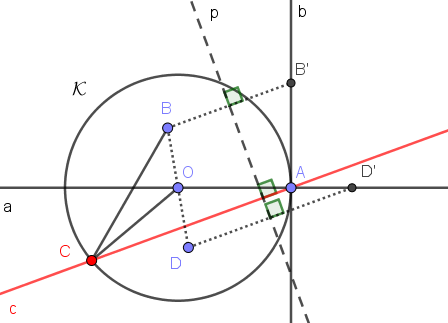
\includegraphics[width=0.6\textwidth]{images/alhazen/scimemi.png}
    \caption[Scimemijeva rešitev]{Scimemijeva rešitev Alhazenovega problema, ko točka $A$ leži na krožnici.}
    \label{fig:scimemi}
\end{figure}

\begin{trditev}
    Točka $C$ je rešitev Alhazenovega problema za točke $O, A, B$.
\end{trditev}
\begin{opomba}
    Avtor je v svoje delo vključil tudi dokaz, vendar je v njem več nejasnosti, priložena skica pa je zavajajoča. Zato tu prilagam svoj dokaz, ki je tudi enostavnejši.
\end{opomba}

\begin{dokaz}
    Naj bo točka $A'$ zrcalna slika točke $A$ čez pregib $p$. Zarišemo še daljici $BA'$ in $DA'$. Potem zaradi simetrije čez pregib $p$ velja $\angle BA'D = \angle B'AD' = 90^\circ$ (slika~\ref{fig:scimemi_dokaz} levo).

    Naj bo $S$ presečišče premice $CO$ z daljico $A'B$. Ker točki $P$ in $A$ ležita na krožnici $\mathcal{K}$, je trikotnik $\triangle CAO$ z vrhom v središču $O$ enakokrak. Sledi $\angle OCA = \angle CAO = \angle CA'D$. Zadnja enakost sledi iz sovršnih kotov ob točki $A$ in simetrije čez pregib $p$. Torej sta kota z vrhom v točkah $P$ in $A'$ (na sliki~\ref{fig:scimemi_dokaz} desno) izmenična, iz česar sledi $CS \parallel DA'$. Zato velja $\angle OSB = \angle DA'B = 90^\circ$.

    \begin{figure}[h]
        \centering
        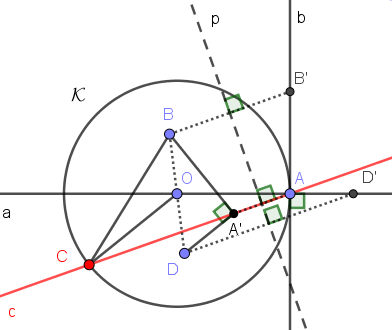
\includegraphics[width=0.47\textwidth]{images/alhazen/scimemi_dokaz1.png}
        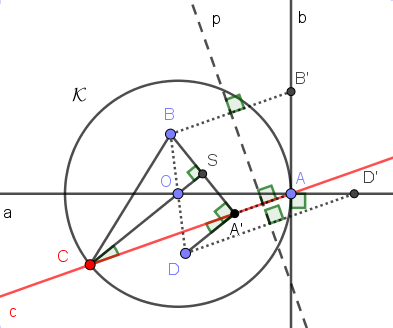
\includegraphics[width=0.47\textwidth]{images/alhazen/scimemi_dokaz2.png}
        \caption[Dokaz Scimemijeve konstrukcije]{Geometrijski dokaz Scimemijeve konstkrukcije}
        \label{fig:scimemi_dokaz}
    \end{figure}

    Trikotnika $\triangle OSB$ in $\triangle DA'B$ sta zato podobna, ker pa je $O$ središče hipotenuze večjega trikotnika, je prvi dvakrat manjši, torej $|BS| = |SA'|$. Zaključimo, da sta zaradi skladnih katet pravokotna trikotnika $\triangle CSB$ in $\triangle CSA'$ skladna, torej res velja $\angle SCB = \angle SCA' = \angle SCA$ oziroma daljica $OC$ res razpolavlja kot $\angle ACB$.
\end{dokaz}

\opomba{Zelo je zanimiv stranski produkt te konstrukcije -- izkaže se namreč, da točke $A, B$ in $E$ (kjer je $E$ drugo presečišče poltraka $PB$ s krožnico $\mathcal{K}$, gl.\ sliko~\ref{fig:scimemi_opomba}) ter njihove slike vse ležijo na isti krožnici! Središče te krožnice pa je presečišče poltraka $CO$ s pregibom $p$. Prav tako velja $BA' \parallel EA$ in $|BE| = |A'A|$. Dokaz za to nalogo ni ključen in ga prepuščamo bralcu.}

\begin{figure}[h]
    \centering
    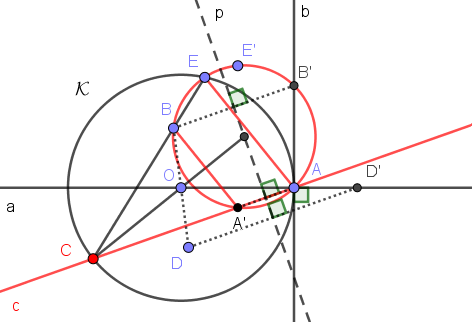
\includegraphics[width=0.6\textwidth]{images/alhazen/scimemi_stransko.png}
    \caption[Stranski produkt Scimemija]{Stranski produkti Scimemijeve konstrukcije točke $P$ (označeno z rdečo).}
    \label{fig:scimemi_opomba}
\end{figure}

\subsubsection*{Huygensova rešitev in Nishimurijev origami postopek}

Nishimura v~\cite{nishimura2018} povzema, kako je Huygens preko kompleksnih števil Alhazenov problem prevedel na iskanje presečišča krožnice z določeno hiperbolo, nekaj več razlage pri izpeljavi pa opiše tudi Alperin v~\cite{alperin2002}. Nishimura od tu nadaljuje v smer, ki nam sproducira konstrukcijo rešitve z origamijem -- vemo že, da presečišče dveh stožnic v projektivni ravnini korespondira s skupno tangento njunih dualnih stožnic, ki smo jih spoznali v razdelku~\ref{podpogl:stoznice_projektivna}. Po novi prevedbi problema na iskanje skupne tangente na dve stožnici avtor svoj članek zaključi še z navedbo origami konstrukcije, ki konstruira rešitev Alhazenovega problema.

V nadaljevanju privzamemo avtorjeve oznake objektov, ki pa se od dosedanjih ne razlikujejo veliko. Brez škode za splošnost naj bo $\mathcal{C}$ enotska krožnica s središčem $O$. Znotraj nje izberemo poljubni točki $A$ in $B$ taki, da so točke $A,B,O$ paroma različne (slika~\ref{fig:huygens1}). Išemo točko $P \in \mathcal{C}$, da bo veljalo
\begin{equation}
    \label{eq:huygens_pogoj}
    \angle APO = \angle OPB.
\end{equation}

\begin{figure}[h]
    \centering
    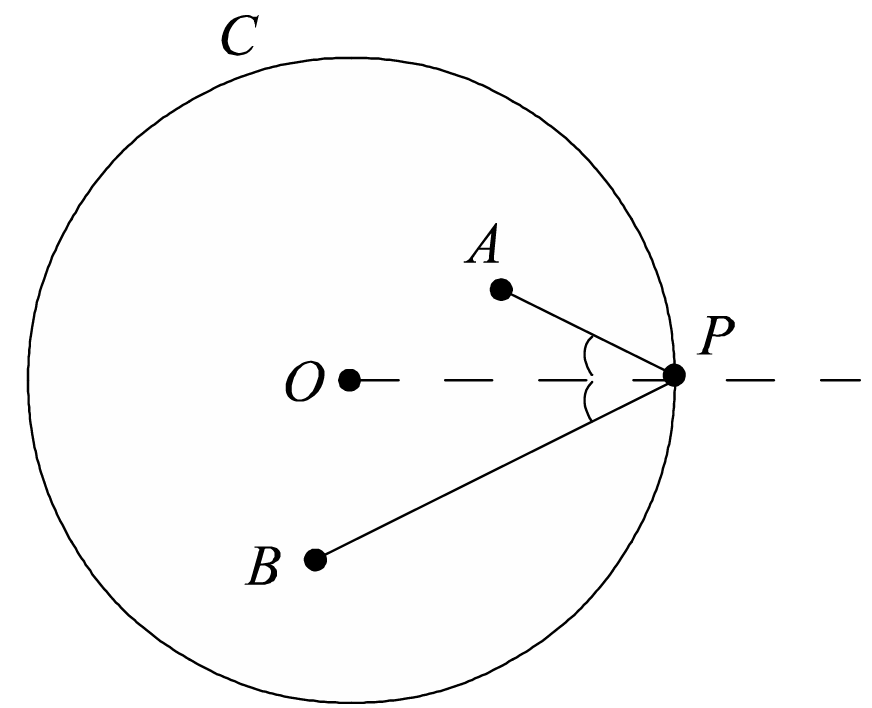
\includegraphics[width=0.35\textwidth]{images/alhazen/huygens1.png}
    \caption[Nastavek Huygensovega reševanja]{Vprašanje Alhazenovega problema. Vzeto iz~\cite[str.\ 37]{nishimura2018}.}
    \label{fig:huygens1}
\end{figure}

Iz pogoja~\ref{eq:huygens_pogoj} za točko $P$ bomo izrazili enačbo stožnice, ki v točki $P$ seka krožnico $\mathcal{C}$. Poslužimo se kompleksnih števil in z njimi izrazimo oba skladna kota. Naj bodo $a, b, z$ kompleksna števila, ki jih zaporedoma ponazarjajo točka $A, B, P$. Potem je kot $\angle APO$ enak kotu med številoma $a-z$ in $-z$, kot $\angle OPB$ pa kotu med številoma $b-z$ in $-z$. Kot med dvema kompleksnima številoma je argument njunega količnika (to sledi iz polarnega zapisa kompleksnih števil), zato pogoj~\ref{eq:huygens_pogoj} preoblikujemo v
$$ \arg \left(\frac{a-z}{-z}\right) = \arg \left(\frac{-z}{b-z}\right). $$
Če delimo kompleksni števili z enakima argumentoma, se njuna kota odštejeta v $0$, torej dobimo realno število. Njegovo konjugirano število mu je torej enako. Zato velja enačba
\begin{equation*}
    \left(\frac{a-z}{-z}\right) \left(\frac{-z}{b-z}\right)^{-1} = \overline{\left(\frac{a-z}{-z}\right) \left(\frac{-z}{b-z}\right)^{-1}}.
\end{equation*}
Enačbo poenostavimo in z upoštevanjem $z \overline{z} = 1$ (ker je $z$ na enotski krožnici) dobimo
\begin{equation}
    \label{eq:huygens_kompleksna_enacba}
    (ab) \overline{z}^2 - (\overline{ab}) z^2 = (a+b) \overline{z} - (\overline{a+b}) z.
\end{equation}
Naj bodo $q, p, r, s, x, y \in \R$ taka števila, da velja
\begin{align*}
    ab &= q + i p, \\
    a + b &= r + i s, \\
    z &= x_0 + i y_0.
\end{align*}
Z upoštevanjem tega se nam enačba~\ref{eq:huygens_kompleksna_enacba} preoblikuje v
\begin{equation*}
    px_0^2 -2qx_0y_0 -py_0^2 - sx_0 + ry_0 = 0.
\end{equation*}
Ker sta koeficienta ob kvadratnih členih različno predznačena, je to enačba hiperbole. Torej je točka $P$ presečišče krožnice~$\mathcal{C}$ in te hiperbole (slika~\ref{fig:huygens2}). Hungerbühler v~\cite{hungerbuhler1992} dobljeno hiperbolo bolj podrobno določi, vendar to za nas ni ključno. 

\begin{figure}[h]
    \centering
    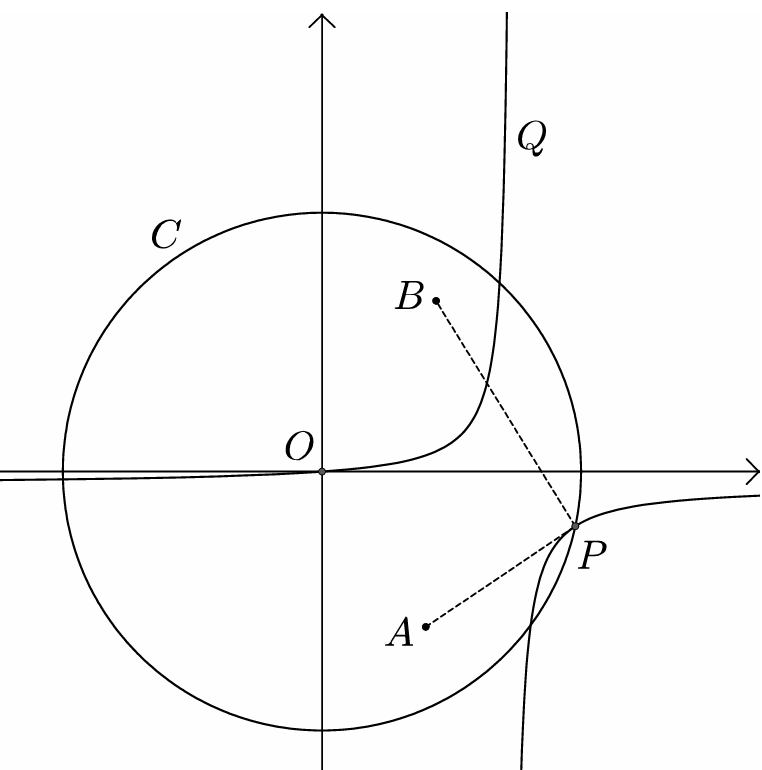
\includegraphics[width=0.4\textwidth]{images/alhazen/huygens2.png}
    \caption[Huygensova rešitev]{Rešitev Alhazenovega problema kot presečišče krožnice in hiperbole. Vzeto iz~\cite[str.\ 39]{nishimura2018}.}
    \label{fig:huygens2}
\end{figure} 

Z origamijem v splošnem ne znamo konstruirati presečišč dveh stožnic, zmoremo pa konstruirati skupne tangente za nekatere primere (do sedaj smo si konkretno pogledali konstrukcije v primeru dveh parabol ter parabole in krožnice, če pri slednjem dovolimo uporabo šestila).

Za lažje nadaljnje reševanje bomo najprej malo poenostavili enačbo dobljene hiperbole. Zavrtimo krožnico $\mathcal{C}$ (in s tem tudi točki $A$ in $B$ znotraj nje) okoli središča $O$ tako, da abscisna os razpolavlja kot $\angle AOB$. S tem na splošnosti nismo izgubili. V tem primeru velja $b = k \cdot \overline{a}$ za nek $k > 0$. Potem je $ab = k \cdot a \overline{a} \in \R$, torej je $p = Im(ab) = 0$.

Torej iščemo presečišče krožnice $\mathcal{C}$ in hiperbole $\mathcal{Q}$ z naslednjima enačbama:
$$ \mathcal{C}: x^2 + y^2 - 1 = 0 \; \text{ in } \; \mathcal{Q}: 2qxy + sx - ry = 0. $$

Vemo že, da je iskanje skupne tangente na dve stožnici ekvivalentno iskanju skupnih točk njunih dualnih stožnic. Zaradi dualnosti tudi skupni točki dveh stožnic ponazarjata skupni tangenti njunih dualnih stožnic.

Bralcu za vajo prepuščamo računanje dualnih stožnic $\mathcal{\overline{C}}$ in $\mathcal{\overline{Q}}$ (gl.\ klasifikacijo stožnic z matriko v razdelku~\ref{podpogl:stoznice_projektivna}). Dobimo
$$ \mathcal{\overline{C}}: x^2 + y^2 - 1 = 0 \; \text{ in } \; \mathcal{\overline{Q}}: r^2x^2 + 2rsxy + s^2y^2 + 4qrx - 4qsy + 4q^2 = 0. $$

\begin{opomba}
    Za izračun dualne stožnice $\mathcal{\overline{Q}}$ je potrebna predpostavka $qrs \neq 0$. Če pa je katero od števil $q, r, s$ ničelno, je hiperbola izrojena, torej se nam problem zreducira na iskanje skupnih presečišč krožnice in dveh premic, kar je računsko zelo enostavno in nas zato ne zanima.
\end{opomba}

Dualna krožnica enotske krožnice je torej prav tako enotska krožnica, stožnica $\mathcal{\overline{Q}}$ pa je parabola (ker je $r^2 \cdot s^2 - \frac{(2rs)^2}{4} = 0$, tj.\ glavni minor pripadajoče matrike je ničeln). Problem je sedaj preveden na iskanje skupne tangente na krožnico $\mathcal{C}$ in parabolo $\mathcal{\overline{Q}}$. To nas razveseli, saj to z origamijem zmoremo storiti.

Kako pa bomo iz skupne tangente določili točko $P$? Iz originalnega iskanja skupne točke $P \in \mathcal{C} \cap \mathcal{Q}$ preidemo na iskanje skupne tangente $\mathcal{\overline{P}} \in \mathcal{\overline{C}} \cap \mathcal{\overline{Q}}$. Ker je $\mathcal{C} = \mathcal{\overline{C}}$, je $\mathcal{\overline{P}} \in \mathcal{\overline{C}}$ ravno tangenta na to krožnico v točki $P$. Iskana točka $P$ je torej dotikališče skupne tangente s krožnico $\mathcal{C}$. Zdaj moramo samo še določiti gorišče in premico vodnico parabole $\mathcal{\overline{Q}}$.

\begin{trditev}
    \label{trd:alh_parab_enacba}
    Parabola $\mathcal{\overline{Q}}$ z enačbo $r^2x^2 + 2rsxy + s^2y^2 + 4qrx - 4qsy + 4q^2 = 0$ ima gorišče $F = \left( \frac{-2qr}{r^2+s^2}, \frac{2qs}{r^2+s^2} \right)$ in premico vodnico $D: sx-ry = 0$.
\end{trditev}
\begin{dokaz}
    Naj bo $X = (x_0, y_0)$ točka, ki je enako oddaljena od gorišča $F$ in premice vodnice $D$. Dokazati moramo, da so njene koordinate rešitve enačbe za parabolo $\mathcal{\overline{Q}}$.

    Spomnimo se splošnih formul za razdaljo med točkama ter razdaljo med točko in premico -- pri danih točkah $T_0 = (x_0, y_0), T_1(x_1, y_1)$ in premici $p: ax + by + c = 0$ velja
    $$ d(T_0, T_1) = \sqrt{(x_1-x_0)^2 + (y_1-y_0)^2}, \; d(T_0, p) = \frac{|ax_0+by_0+c|}{\sqrt{r^2+s^2}}.$$
    Tako iz $d(X, F) = d(X, D)$ dobimo enačbo
    $$ \left( x_0 + \frac{2qr}{r^2+s^2} \right)^2 + \left( y_0 - \frac{2qs}{r^2+s^2} \right)^2 = \frac{(sx_0 - ry_0)^2}{r^2+s^2} $$
    Ko izraze na obeh straneh poenostavimo in malo preuredimo enačbo, dobimo $r^2x_0^2 + 2rsx_0y_0 + s^2y_0^2 + 4qrx_0 - 4qsy_0 + 4q^2 = 0$, torej je $\mathcal{\overline{Q}}$ res parabola.
\end{dokaz}

Tako smo prišli do konca teoretičnega postopka. Na hitro ponovimo -- pri dani enotski krožnici $\mathcal{C}$ in točkama $A, B$ znotraj nje (postopek velja tudi za točki zunaj krožnice) nam presečišče $P$ krožnice $\mathcal{C}$ s hiperbolo $\mathcal{Q}$, ki je odvisna od točk $A$ in $B$, reši Alhazenov problem. Presečišče stožnic prevedemo v iskanje skupne tangente $\overline{P}$ na krožnico $\mathcal{C}$ in parabolo $\mathcal{\overline{Q}}$, ki je dualna stožnica hiperbole. Iskana točka $P$ je dotikališče tangente $\overline{P}$ s krožnico $\mathcal{C}$ (slika~\ref{fig:nishimura_resitev}).

\begin{figure}[h]
    \centering
    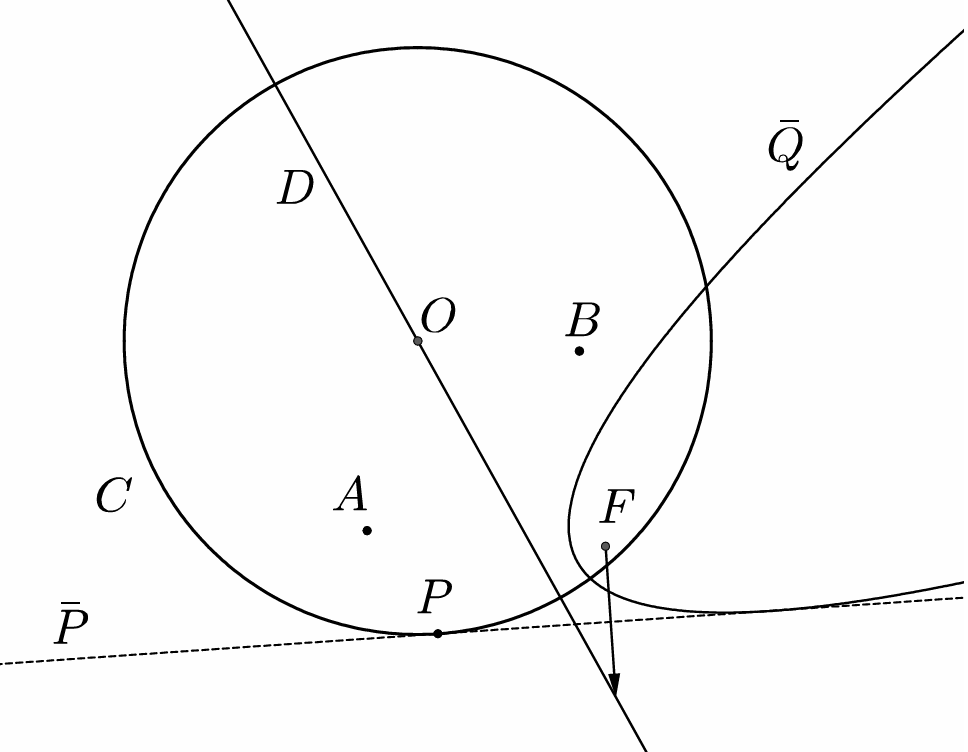
\includegraphics[width=0.5\textwidth]{images/alhazen/nishimura_resitev.png}
    \caption[Nishimurijeva rešitev]{Konstrukcija dotikališča skupne tangente s krožnico. Vzeto iz~\cite[str.\ 40]{nishimura2018}.}
    \label{fig:nishimura_resitev}
\end{figure}

Vemo že, da z evklidskim orodjem problema ne moremo rešiti, saj se prevede na reševanje enačbe četrte stopnje. Ta postopek pa nam še na drug način pokaže potrebnost origamija -- konstrukcija skupne tangente na krožnico in parabolo namreč z neoznačenim ravnilom in šestilom prav tako ni mogoča, spomnimo pa se, da jo lahko dobimo s hkratnim prepogibom središča krožnice na rob dvakrat večje krožnice in gorišča parabole na njeno premico vodnico.

Nishimura vse znanje tega razdelka združi v naslednjo origami konstrukcijo, ki konstruira rešitev Alhazenovega problema. Naj bo $\mathcal{C}$ enotska krožnica s središčem $O$ v koordinatnem izhodišču kompleksne ravnine $\C$ in $a = A, b = B$ točki znotraj nje. Za točki zunaj krožnice je postopek enak.
\begin{enumerate}
    \item Prepognemo poltrak $OA$ in njegovo presečišče s krožnico $\mathcal{C}$ označimo z $E$.
    \item Prepognemo premico $AB$.
    \item Prepognemo simetralo daljice $AB$ in središče daljice $AB$ označimo z $M$. Velja $ |OM| = |(a+b)/2| = \sqrt{s^2+r^2}/2$.
    \item Prepognemo premico $OM$, ki jo poimenujemo $D$ (ker je $ M = (a+b)/2$, je to ravno premica vodnica parabole $\mathcal{\overline{Q}}$). Presečišče poltraka $OM$ s krožnico $\mathcal{C}$ označimo z $E'$.
    \item Prepognemo premico $EB$.
    \item Prepognemo pravokotnico na premico $EB$ skozi točko $B$ in jo poimenujemo $l_1$.
    \item Prepognemo pravokotnico na premico $l_1$ skozi točko $A$ in jo poimenujemo $l_2$. Velja $l_2 \parallel EB$.
    \item Prepognemo premico $OB$ in njeno presečišče s premico $l_2$ označimo z $G$. Iz razmerja podobnih trikotnikov $\triangle AOG$ in $\triangle EOB$ sledi $|OG| = q = Re(ab)$ (slika~\ref{fig:nishimura_origami}).
    \begin{figure}[h]
        \centering
        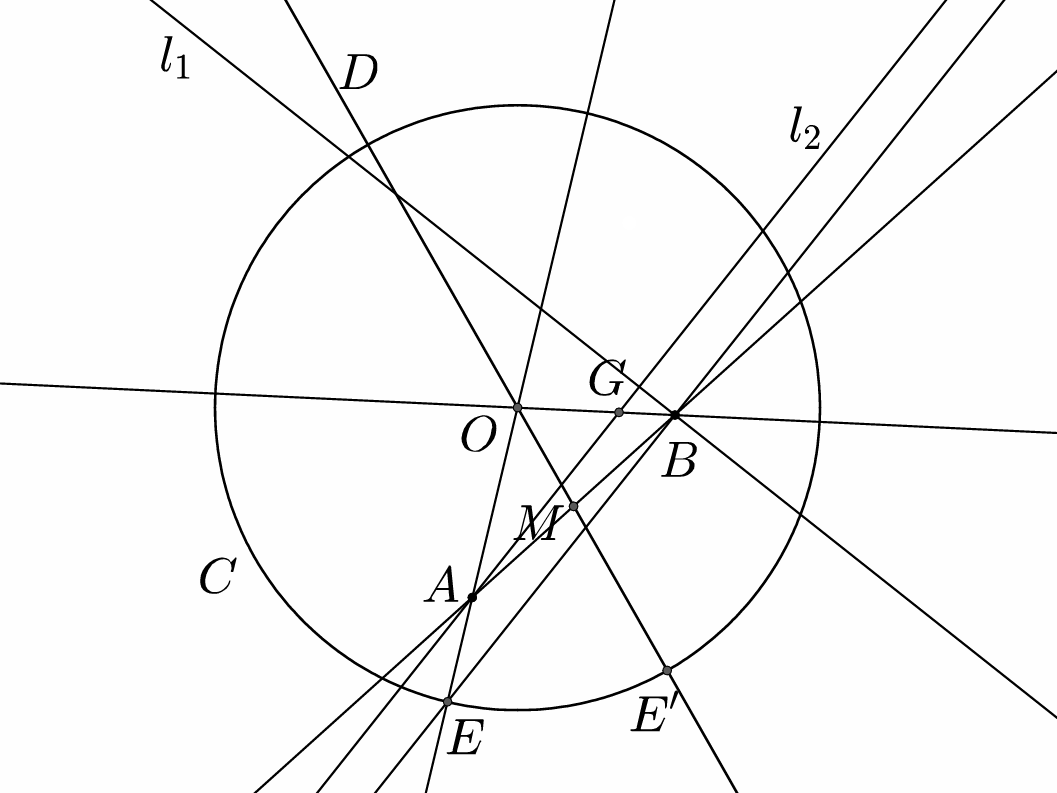
\includegraphics[width=0.6\textwidth]{images/alhazen/nishimura_origami.png}
        \caption[Nishimurijeva konstrukcija $1$]{Nishimurijeva origami konstrukcija do koraka $8$. Vzeto iz~\cite[str.\ 41]{nishimura2018}.}
        \label{fig:nishimura_origami}
    \end{figure}
    \item Prepognemo premico $MG$.
    \item Prepognemo pravokotnico na premico $MG$ skozi točko $M$ in jo označimo z $l_3$.
    \item Prepognemo pravokotnico na premico $l_3$ skozi točko $E'$ in njeno presečišče s premico $OB$ označimo s $H$. Velja $MG \parallel E'H$. Iz razmerja podobnih trikotnikov $\triangle OMG$ in $\triangle OE'H$ sledi $|OH|= |OG|/|OM| = 2q/ \sqrt{s^2+r^2}$.
    \item Prepognemo premico skozi središče $O$, ki točko $H$ preslika na premico $D$ v točko $K$. Velja $|OK| = |OH|$.
    \item Prepognemo premico skozi središče $O$, ki točko $B$ preslika na premico $OA$. To je ravno simetrala kota $\angle AOB$, za katero smo prevzeli, da je to ravno abscisna os v našem koordinatnem sistemu. Sliko točke $K$ čeznjo označimo s $F$ (slika~\ref{fig:nishimura_origami2}).
    
    Ker je premica $OF$ zrcalna slika premice $D$ čez abscisno os, je njena enačba $OF: $. Zaradi simetrije velja $|OF| = |OK| = |OH| = 2q/ \sqrt{s^2+r^2}$. Za točko $F = (x,y)$ tako dobimo sistem enačb
    $$ sx+ry=0 \; \text{ in } \; \sqrt{x^2+y^2} = \frac{2q}{\sqrt{s^2+r^2}},$$
    katerega rešitev so ravno koordinate gorišča iskane parabole iz trditve~\ref{trd:alh_parab_enacba} (lahek izračun je prepuščen bralcu), torej je točka $F$ gorišče parabole $\mathcal{\overline{Q}}$ s premico vodnico $D$.
    
    \item Za določitev iskane točke $P$ samo še prepognemo tangento $\overline{P}$ na krožnico $\mathcal{C}$, ki točko $F$ položi na premico $D$. Točka $P$ je dotikališče tangente $\overline{P}$ s krožnico $\mathcal{C}$ (slika~\ref{fig:nishimura_resitev}).
    \begin{figure}[h]
        \centering
        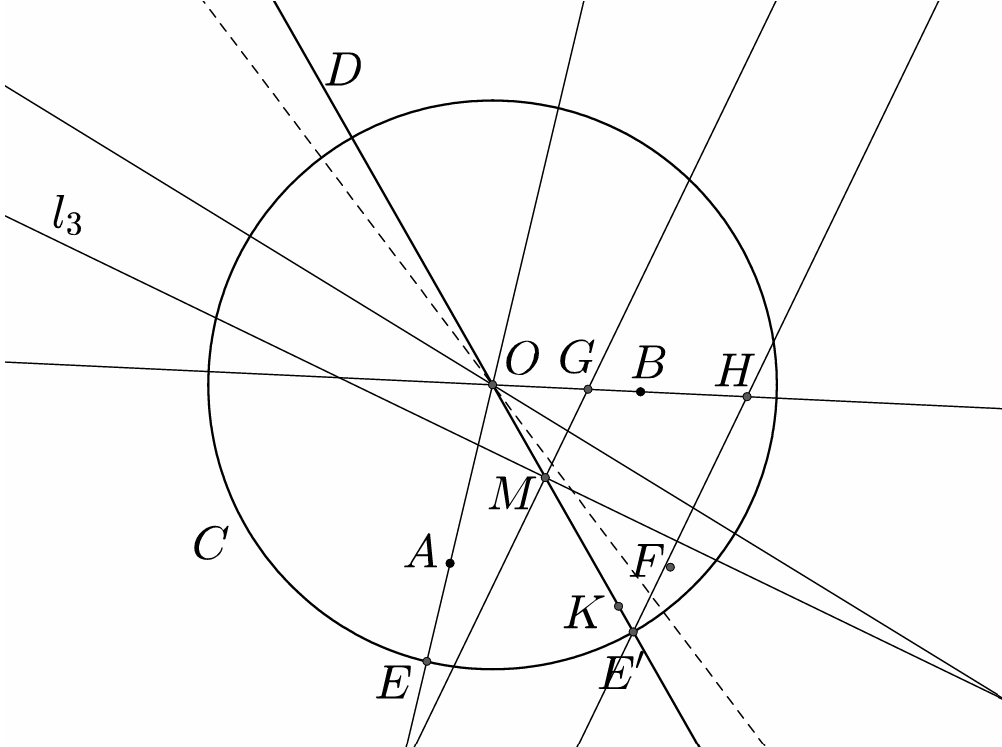
\includegraphics[width=0.6\textwidth]{images/alhazen/nishimura_origami2.png}
        \caption[Nishimurijeva konstrukcija $2$]{Nishimurijeva origami konstrukcija gorišča $F$ (korak $13$). Vzeto iz~\cite[str.\ 42]{nishimura2018}.}
        \label{fig:nishimura_origami2}
    \end{figure}
\end{enumerate}